% !TeX program = pdflatex
% Standalone source. Compile with pdfLaTeX; no external figures are required.
\documentclass[11pt,a4paper]{article}
\usepackage[margin=20mm]{geometry}
\usepackage[T1]{fontenc}
\usepackage{lmodern}
\usepackage{amsmath,amssymb,booktabs,array,xcolor,tikz,fancyhdr,hyperref,listings,pgfplots}
\usetikzlibrary{calc,arrows.meta}
\hypersetup{colorlinks=true,linkcolor=blue!50!black,urlcolor=blue!50!black}
\definecolor{accent}{HTML}{124E66}
\definecolor{pcol}{HTML}{A24021}
\definecolor{ncol}{HTML}{175A86}
\pagestyle{fancy}\fancyhf{}\fancyhead[L]{\small EE3032 / Fall 2021 / HW2}
\fancyhead[R]{\small CMOS logic}\fancyfoot[C]{\thepage}
\setlength{\headheight}{15pt}\setlength{\parindent}{0pt}\setlength{\parskip}{6pt}
\renewcommand{\arraystretch}{1.2}
\newcommand{\answer}[1]{\par\noindent\colorbox{accent!9}{\parbox{0.96\linewidth}{#1}}\par}
\newcommand{\AND}{\,}
\newcommand{\VDD}{V_{\mathrm{DD}}}
\newcommand{\VSS}{V_{\mathrm{SS}}}
% A conventional switch-level MOS symbol: continuous channel, insulated gate,
% and a gate bubble for pMOS. Bulk terminals are omitted, as explained below.
% Arguments: device id, x, y, gate literal, p or n. t/b are upper/lower terminals.
\newcommand{\MOS}[5]{
  \coordinate (#1) at (#2,#3);
  \coordinate (#1t) at ($(#1)+(0,.55)$);
  \coordinate (#1b) at ($(#1)+(0,-.55)$);
  \draw (#1t)--($(#1)+(0,.30)$)--($(#1)+(-.18,.30)$);
  \draw ($(#1)+(-.18,.34)$)--($(#1)+(-.18,-.34)$);
  \draw ($(#1)+(-.18,-.30)$)--($(#1)+(0,-.30)$)--(#1b);
  \draw ($(#1)+(-.35,.33)$)--($(#1)+(-.35,-.33)$);
  \def\type{#5}\def\ptype{p}
  \ifx\type\ptype
    \draw ($(#1)+(-.78,0)$)--($(#1)+(-.53,0)$);
    \draw ($(#1)+(-.465,0)$) circle (.065);
    \draw ($(#1)+(-.40,0)$)--($(#1)+(-.35,0)$);
  \else
    \draw ($(#1)+(-.78,0)$)--($(#1)+(-.35,0)$);
  \fi
  \node[anchor=east] at ($(#1)+(-.82,0)$) {$#4$};
  \node[anchor=west,font=\scriptsize] at ($(#1)+(.10,0)$) {#1};
}
% A transmission-gate instance; its two MOS devices are expanded on page 3.
\newcommand{\TG}[4]{
  \node[draw,rounded corners=1pt,minimum width=11mm,minimum height=6mm,
        fill=accent!5,font=\small] (#1) at (#2,#3) {$\mathrm{TG}_{#4}$};
}

\pgfplotsset{compat=1.18}
\lstset{basicstyle=\ttfamily\scriptsize,breaklines=true,frame=single,columns=fullflexible}
\begin{document}
\begin{center}{\LARGE\bfseries 2021 HW2}\\[4pt]{\large Dual Thresholds, a Rotator, and Ratioed Logic}\\[4pt]{\small EE3032 / Introduction to VLSI Design}\end{center}
\textbf{Provenance.} The original assignment and the supplied answers by Lin Yan-Yu were read first. The results below were independently derived, with the useful reference choices retained and improvements identified. Source details and hashes are in the year-level \texttt{SOURCES.md}.


\section*{1. High-$V_t$ selection on the NAND branch}
From the original gate symbols,
\[
 D=\bar A\oplus B=AB+\bar A\bar B,\qquad E=\overline{BC}.
\]
With the given one-unit low-$V_t$ gate model, the path $A\to inverter\to XOR\to D$ is critical at two units. The direct $B\to XOR\to D$ and the two NAND paths each take one unit. Keep the inverter and XOR realization low-$V_t$; replace the \emph{entire} NAND driving $E$ by high-$V_t$ devices.
\begin{center}\begin{tabular}{lccc}\toprule
Path&Low-$V_t$ delay&New delay&Slack before change\\\midrule
$A\to D$&2&2&0\\$B\to D$&1&1&1\\$B,C\to E$&1&$d_{\rm HVT,NAND}$&1\\\bottomrule
\end{tabular}\end{center}
\textbf{Necessary timing condition:} $d_{\rm HVT,NAND}\le2$ units. The prompt supplies no high-$V_t$ delay or threshold values, so a numerical leakage reduction or unconditional timing guarantee cannot be inferred. Size the high-$V_t$ NAND if necessary to satisfy this condition. Changing transistors inside the shared critical XOR without a library timing model is not justified by the direct-$B$ slack alone.
Below is a fully complementary static-CMOS realization. Complement-driver outputs are labeled rather than routed across the schematic; connect each identically named gate to its driver. All pMOS bodies connect to VDD and all nMOS bodies to VSS. The B complement generator belongs to the XOR-cell implementation, within the given abstract cell-delay model.
\begin{center}
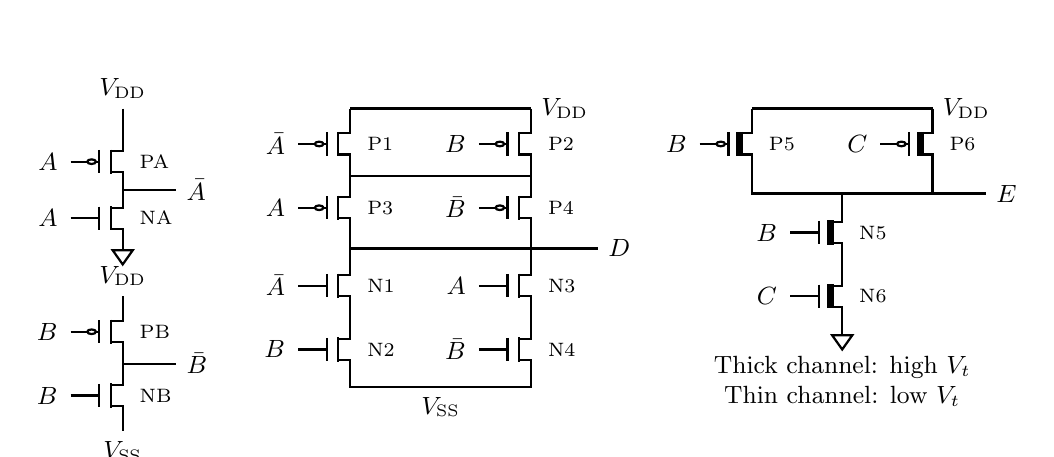
\begin{tikzpicture}[x=.85cm,y=.45cm,line width=.8pt,font=\small]
% Thin-channel low-Vt devices.
\MOS{P1}{0}{6.5}{\bar A}{p}\MOS{P2}{2.7}{6.5}{B}{p}
\MOS{P3}{0}{4.7}{A}{p}\MOS{P4}{2.7}{4.7}{\bar B}{p}
\draw (0,7.5)--(2.7,7.5) node[right] {$\VDD$};
\draw (0,7.5)--(P1t) (2.7,7.5)--(P2t);
\draw (P1b)--(0,5.6)--(2.7,5.6)--(P2b);
\draw (0,5.6)--(P3t) (2.7,5.6)--(P4t);
\draw (P3b)--(0,3.55)--(3.7,3.55) node[right] {$D$};\draw (P4b)--(2.7,3.55);
\MOS{N1}{0}{2.5}{\bar A}{n}\MOS{N2}{0}{.7}{B}{n}
\MOS{N3}{2.7}{2.5}{A}{n}\MOS{N4}{2.7}{.7}{\bar B}{n}
\draw (0,3.55)--(N1t) (2.7,3.55)--(N3t) (N1b)--(N2t) (N3b)--(N4t);
\draw (N2b)--(0,-.35)--(2.7,-.35)--(N4b);\node[below] at (1.35,-.35) {$\VSS$};
% Two low-Vt complement drivers.
\MOS{PA}{-3.4}{6.0}{A}{p}\MOS{NA}{-3.4}{4.4}{A}{n}
\draw (-3.4,7.5) node[above] {$\VDD$}--(PAt) (PAb)--(NAt);
\draw (-3.4,5.2)--(-2.6,5.2) node[right] {$\bar A$};\draw (NAb)--(-3.4,3.5);\draw (-3.55,3.5)--(-3.25,3.5)--(-3.4,3.1)--cycle;
\MOS{PB}{-3.4}{1.2}{B}{p}\MOS{NB}{-3.4}{-.6}{B}{n}
\draw (-3.4,2.2) node[above] {$\VDD$}--(PBt) (PBb)--(NBt);
\draw (-3.4,.3)--(-2.6,.3) node[right] {$\bar B$};\draw (NBb)--(-3.4,-1.6) node[below] {$\VSS$};
% The E NAND uses thick-channel high-Vt devices.
\MOS{P5}{6.0}{6.5}{B}{p}\MOS{P6}{8.7}{6.5}{C}{p}
\MOS{N5}{7.35}{4.0}{B}{n}\MOS{N6}{7.35}{2.2}{C}{n}
\draw (6,7.5)--(8.7,7.5) node[right] {$\VDD$};\draw (6,7.5)--(P5t) (8.7,7.5)--(P6t);
\draw (P5b)--(6,5.1)--(9.5,5.1) node[right] {$E$};\draw (P6b)--(8.7,5.1);
\draw (7.35,5.1)--(N5t) (N5b)--(N6t);\draw (N6b)--(7.35,1.1);\draw (7.2,1.1)--(7.5,1.1)--(7.35,.7)--cycle;
\foreach \x/\y in {6/6.5,8.7/6.5,7.35/4,7.35/2.2}{\draw[line width=2.5pt] (\x-.18,\y+.34)--(\x-.18,\y-.34);}
\node[align=center] at (7.35,-.2) {Thick channel: high $V_t$\\Thin channel: low $V_t$};
\end{tikzpicture}\end{center}
\textbf{Reference comparison.} The supplied answer selects the NAND branch for high $V_t$ correctly. We retain that choice and state the missing timing assumption. The netlist \texttt{dual\_vt\_logic.sp} exposes symbolic LVT/HVT models; CIC018 TT does not supply this dual-$V_t$ PDK. Eight exhaustive Boolean tests pass. The runnable \texttt{dual\_vt\_boolean\_testbench.sp} additionally checks all eight states using explicitly illustrative Level-1 models; it does not verify dual-$V_t$ process leakage or timing.
\newpage
\section*{2. Active-low one-hot cyclic rotator}
Only the four listed control words are specified. Let $r=0,1,2,3$ when $c_{3-r}=0$ and the other controls are one. Then
\[
 \boxed{z_j=a_{(j-r)\bmod4}},\quad j=0,1,2,3.
\]
Under that legal-control assumption, the direct sum of selected paths is
\[
 z_j=\bar c_3a_j+\bar c_2a_{(j-1)\bmod4}
      +\bar c_1a_{(j-2)\bmod4}+\bar c_0a_{(j-3)\bmod4}.
\]
\begin{center}\begin{tabular}{c|cccc|c}\toprule
$c_3c_2c_1c_0$&$z_3$&$z_2$&$z_1$&$z_0$&$r$\\\midrule
0111&$a_3$&$a_2$&$a_1$&$a_0$&0\\
1011&$a_2$&$a_1$&$a_0$&$a_3$&1\\
1101&$a_1$&$a_0$&$a_3$&$a_2$&2\\
1110&$a_0$&$a_3$&$a_2$&$a_1$&3\\\bottomrule
\end{tabular}\end{center}
Generate the four $\bar c_i$ values once with CMOS inverters. For each output $z_j$, connect four transmission gates in parallel. Path $r$ connects $a_{(j-r)\bmod4}$ to $z_j$, using nMOS gate $\bar c_{3-r}$ and pMOS gate $c_{3-r}$. Exactly one path is on for every specified control word.
\begin{center}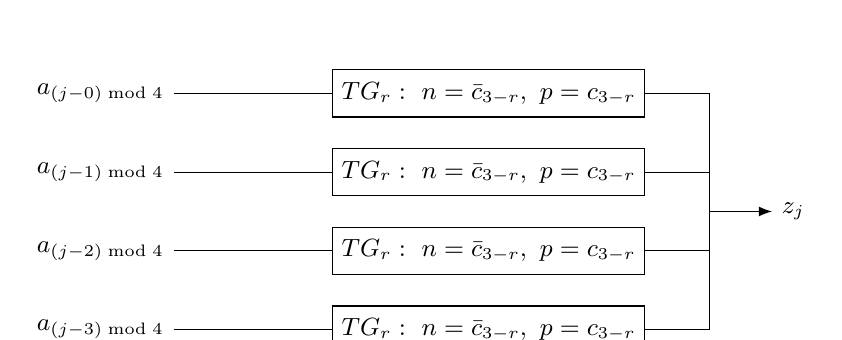
\begin{tikzpicture}[>=Latex,font=\small]
\foreach \r/\y in {0/3,1/2,2/1,3/0}{
\node[draw,minimum width=33mm,minimum height=6mm] (t\r) at (0,\y) {$TG_r:\ n=\bar c_{3-r},\ p=c_{3-r}$};
\draw (-4.0,\y) node[left] {$a_{(j-\r)\bmod4}$}--(t\r.west);
\draw (t\r.east)--(2.8,\y);
}
\draw (2.8,0)--(2.8,3);\draw[->] (2.8,1.5)--(3.6,1.5) node[right] {$z_j$};
\end{tikzpicture}\end{center}
\textbf{Transmission-gate transistor expansion:} each box contains two MOSFETs with the same data terminals, shown below. The small pMOS gate bubble denotes active-low conduction.
\begin{center}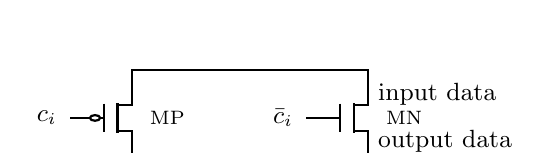
\begin{tikzpicture}[x=1cm,y=.55cm,line width=.8pt,font=\small]
\MOS{MP}{0}{1}{c_i}{p}\MOS{MN}{3}{1}{\bar c_i}{n}
\draw (MPt)--(0,2.1)--(3,2.1)--(MNt) node[right] {input data};
\draw (MPb)--(0,-.1)--(3,-.1)--(MNb) node[right] {output data};
\end{tikzpicture}\end{center}
There are $4\times4\times2=32$ pass transistors plus eight inverter transistors: \textbf{40 transistors}. A data path crosses one TG and passes full rail voltages. Multiple zero controls would connect distinct input sources together, and all-one controls disconnect the outputs; these patterns are outside the specified domain.
\textbf{Reference comparison.} The supplied schematic decodes each four-bit control word with four serial TGs per input path. It is valid for the listed controls, but has more devices and four pass stages. The direct one-hot implementation above is smaller. \texttt{verify\_logic.py} and actual CIC018 HSPICE both pass all $16\times4=64$ cases (256 output-bit checks), with 1 fF on each output.
\newpage
\section*{3. Pseudo-NMOS NOR and its size constraint}
The pull-up pMOS has a grounded gate and is always on. The two parallel nMOS devices form the pull-down OR network. Hence
\[
 \boxed{V_o=\overline{A+B}}.
\]
\begin{center}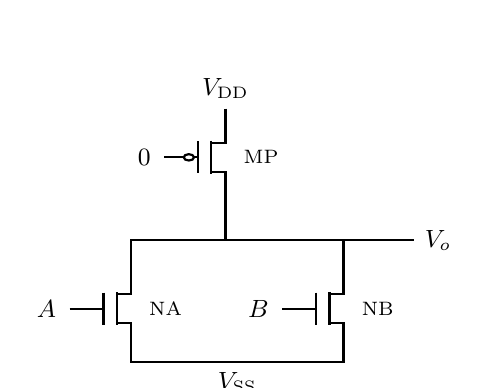
\begin{tikzpicture}[x=1cm,y=.62cm,line width=.8pt,font=\small]
\MOS{MP}{0}{5.2}{0}{p}\MOS{NA}{-1.2}{2.1}{A}{n}\MOS{NB}{1.5}{2.1}{B}{n}
\draw (0,6.2) node[above] {$\VDD$}--(MPt);
\draw (MPb)--(0,3.5)--(-1.2,3.5)--(NAt);\draw (0,3.5)--(2.4,3.5) node[right] {$V_o$};\draw (1.5,3.5)--(NBt);
\draw (NAb)--(-1.2,1)--(1.5,1)--(NBb);\node[below] at (.15,1) {$\VSS$};
\end{tikzpicture}\end{center}
Let $s_n$ and $s_p$ multiply the common reference aspect ratio $W/L$. By the specified constant-resistance model,
\[
 R'_n=R_n/s_n,\qquad R'_p=R_p/s_p=2R_n/s_p.
\]
The worst low level is when exactly one nMOS is on; two on devices halve the pull-down resistance. Thus
\[
 V_{OL,\max}=\VDD\frac{R'_n}{R'_p+R'_n}\le0.1\VDD
 \iff R'_p\ge9R'_n
 \iff \boxed{s_n\ge\tfrac92 s_p.}
\]
Both nMOS must satisfy this bound independently. With equal lengths choose $(W/L)_n=4.5(W/L)_p$. Equivalently choose $s_n=9,s_p=2$, as in the supplied answer. The ratio is $\ge4.5$, not a required absolute transistor width.
For $R_n=1\,\mathrm{k}\Omega$, $s_n=9,s_p=2$, and $\VDD=1.8$ V:
\begin{center}\begin{tabular}{cc|cc}\toprule
$A$&$B$&Constant-R $V_o$ (V)&Actual CIC018 TT $V_o$ (V)\\\midrule
0&0&1.800000&1.800000\\0&1&0.180000&0.030165\\
1&0&0.180000&0.030122\\1&1&0.094737&0.014822\\\bottomrule
\end{tabular}\end{center}
\textbf{Physical check.} \texttt{pseudo\_nor.sp} chooses $W_p=1\,\mu$m, $W_n=4.5\,\mu$m, and $L=0.18\,\mu$m. Real HSPICE at TT, $25^\circ$C, and 1.8 V meets the $0.18$ V low-level bound. BSIM is not the prompt's constant-R model, so the smaller observed values are supplementary process-specific results, not an alternative derivation. Ratioed logic dissipates static current when pulled low.
\textbf{Reference comparison.} The supplied Boolean NOR and $(s_n,s_p)=(9,2)$ selection are correct and retained. This solution states the full inequality and verifies both the specified resistance model and the local process model.
\textbf{Reproduce.} Run \texttt{python verify\_logic.py}, then \texttt{python reproduce.py --model D:/cic018.l --work PATH}. The simulator defaults to the installed HSPICE path and accepts \texttt{--hspice}. Outputs are in \texttt{results/}; raw logs stay in the specified work directory. No process-model text is distributed.
\end{document}
